\section{User Registration Process}
\label{sec:reg}

In general, a user can sign up for a YouPower account at the application's welcome page\footnote{\url{https://app.civisproject.eu/frontend.html}}. In this case, the user can use the Action Suggestion part of the application. For the Housing Cooperative part or the Energy Awareness part of the application, more specific user (and energy) information is needed by the application. There are tailored solutions for the Swedish and the Italian test sites respectively which are presented in the following two subsections. With respect to scalability, similar procedures can be used as a means to enable new/extended features of the application. 

\subsection{Swedish Test Site}

For the Swedish test site users, the registration process depends on the type of user (household member or energy manager) and for household users if their energy data is managed by the cooperative or not (affecting mainly step 2 below). The users register as follows:

\begin{enumerate}
\item A household user receives a flyer with information about the app and a URL (also provided as a QR code) that is housing-cooperative-specific, i.e. the housing cooperative which the user belongs to. 

The URL location is managed by KTH (i.e. it is a local Swedish URL) in the format of  \texttt{\small http://civis.proj.kth.se/}\textit{\{unique-link-of-a-housing-coopertive\}}. Energy managers receive the same URL for their housing cooperative but via email. 

\item For housing cooperatives that manage their own apartment level energy data (i.e. own the apartment level energy meters), the user is provided with a unique code on the flyer that they enter to link their account to the household energy data. Users from housing cooperatives that do not own the apartment level energy meters are asked to enter information from their energy bill, and the flyer specifies where on the bill they can find that information. Energy managers similarly provide information from the housing cooperative energy bill to create housing cooperative level accounts.

\item On the sign-up page (see Figure \ref{fig:signup_s}), the user is asked to fill in email address, name and password to create an account (compulsory information). It is also possible to add household information (optional) about the size of the apartment and number of adults (18 years and above) and children (below 18 years) in the household. The name of the housing cooperative is prefilled. For energy managers, household information is only needed in the cases where the housing cooperatives also have household accounts (at present only applicable for two housing cooperatives).

\begin{figure}[h!]
	\centering
	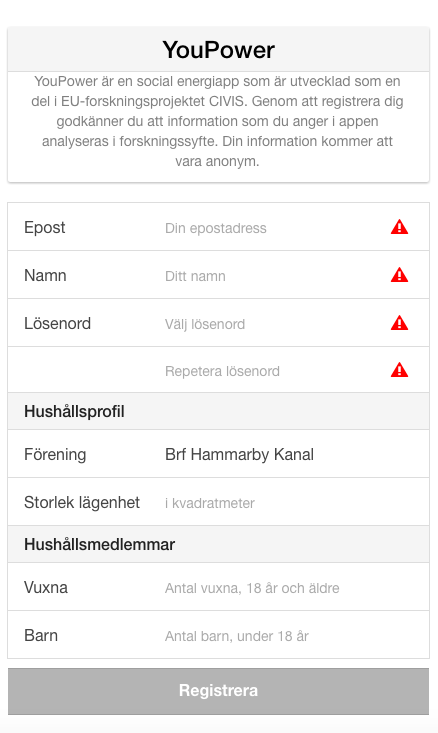
\includegraphics[width=0.45\linewidth]{img/signup_s.png}
	\caption{Sign-up page Swedish test site.}
	\label{fig:signup_s}
\end{figure}

\item By creating an account, the user consents to CIVIS using the data in the app for research purposes. After completing the form, the user is directed to the YouPower app. Energy managers are given editing rights and can choose to add an email address to the energy contact person in the cooperative, update information about the cooperative (number of apartments, type of ventilation etc.) and add energy reduction actions that the cooperative has taken.

\item The flyer recommends the user to use the webapp on a mobile phone and it also gives instructions for how to create a link to the app on the phone's home screen.

\end{enumerate}

\subsection{Italian Test Site}

New Trentino users should follow a 2-step process to sign up YouPower to use the \textit{Energy Data} features.

\begin{enumerate}

\item A user can sign up at YouPower welcome page\footnote{\url{https://app.civisproject.eu/frontend.html}} by filling basic user information such as user name and email address in the sign-up page(see Figure \ref{fig:reg_italian}-1). The user automatically logs into YouPower after successful registration.

\item In order to access the functionalities discussed in Sec.~\ref{sec:energydata}, Italian users should provide a valid \textit{ContractID} and \textit{TestbedID} in the app \textit{Settings} page (see Figure \ref{fig:reg_italian}-2). The ContractID will be matched to an \textit{ApartmentID} of the household to access the energy data from the back-end while the testbed location will be used to fetch community related information like ToU signals in the municipality and total consumption of the test site. 
\begin{figure}
      \begin{center}
        \begin{minipage}[htb]{0.45\linewidth}    
         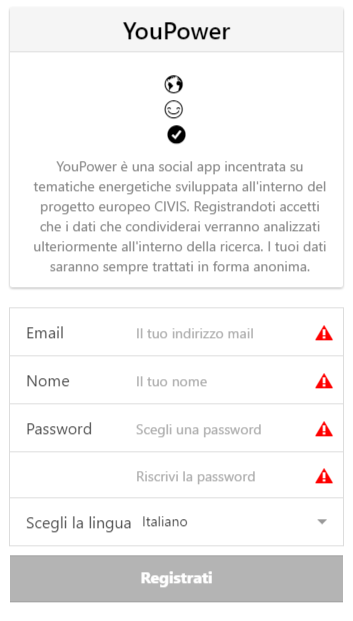
\includegraphics[width=1\linewidth]{img/registrationpart.png}  
        \end{minipage}
 	\hfill 
        \begin{minipage}[htb]{0.45\linewidth}    
         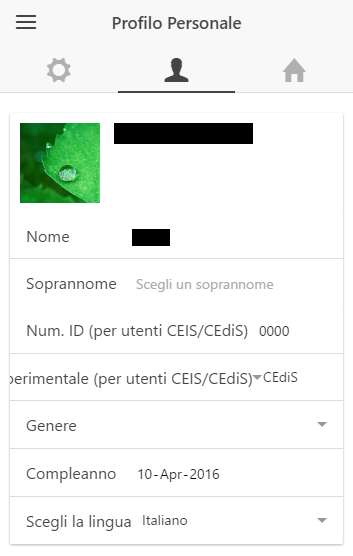
\includegraphics[width=1\linewidth]{img/Italiansettings.png}  
        \end{minipage}
      \end{center}
    \caption{(1) Sign-up page for Italian test site (2) Settings page for Italian test site users.
}
\label{fig:reg_italian}
\end{figure}

After this step, the \textit{Energy Data} tab of YouPower will be activated for Italian users.
\end{enumerate}